\documentclass[french]{article}
\usepackage{aeguill,aecompl,babel,tikz,geometry}
\usetikzlibrary{arrows} % package de flèches
\usepackage[T1]{fontenc}
\usepackage[utf8]{inputenc}
\pagestyle{empty}
\geometry{
paperwidth=20cm,
paperheight = 11cm,
left=0pt,
right=0pt,
top=2pt,
bottom=0pt
}
%\tikzset{%
%cat/.style={right=2cm,anchor=west,align=left},
%subcat/.style={below=1cm,anchor=north west,draw=none,font=\em,align=left}
%}
%\pgfdeclarelayer{background}
%\pgfsetlayers{background,main}

\begin{document}
\centering

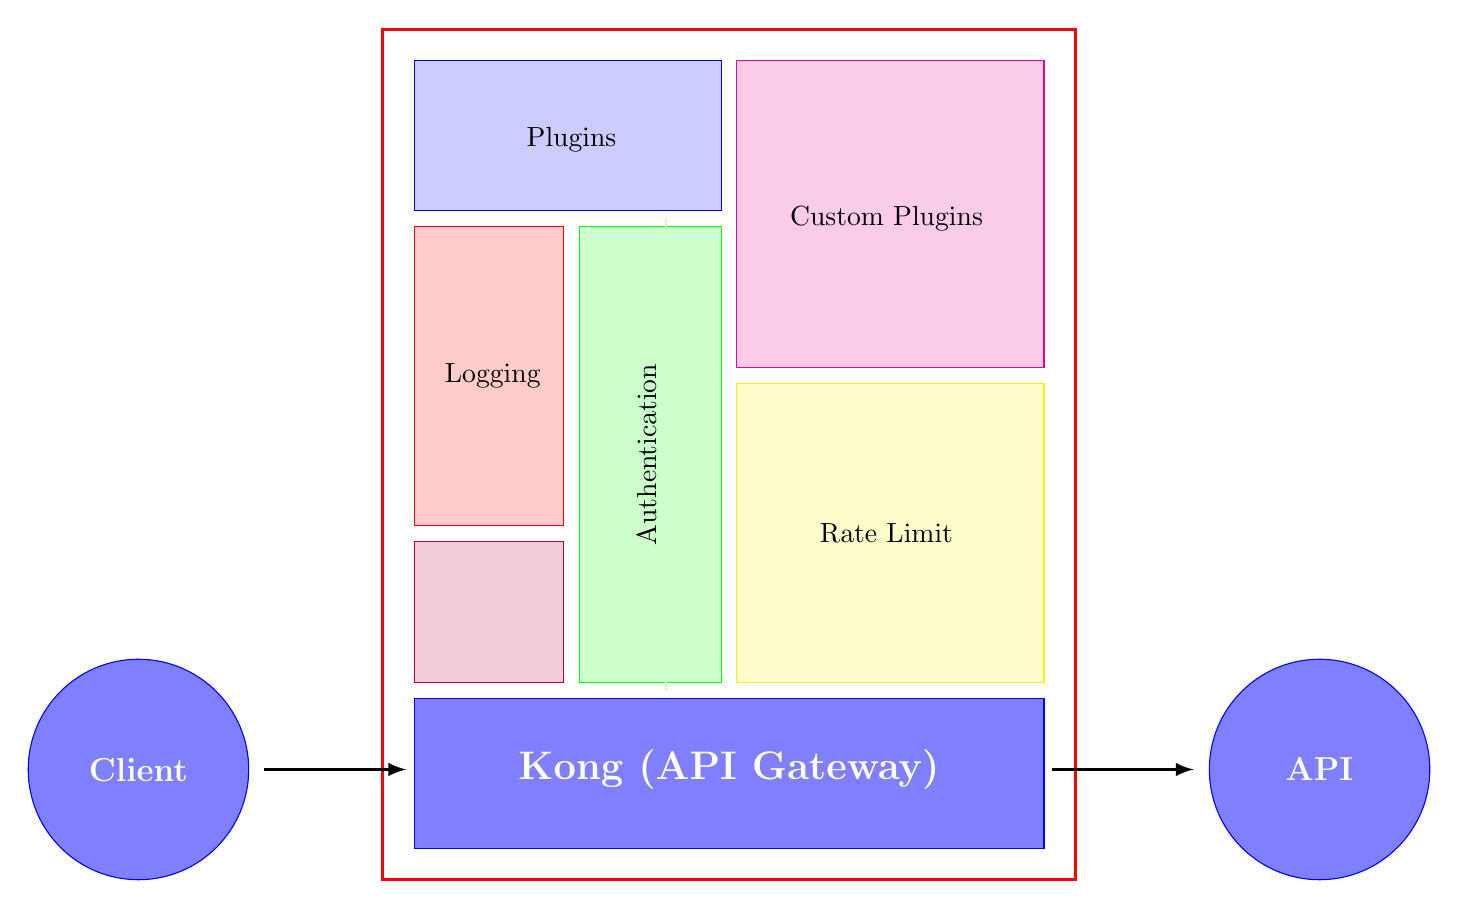
\begin{tikzpicture}

\draw [red, very thick] (4.6,10.4) rectangle (13.4,-0.4);

\draw [blue,fill=blue!50] (5,1.9) rectangle (13,0);
\draw (9,1) node[white] {\Large{\textbf{Kong (API Gateway)}}};

\draw [purple,fill=purple!20] (5,3.9) rectangle (6.9,2.1);

\draw [green,fill=green!20] (7.1,7.9) rectangle (8.9,2.1);
\draw [green!20] (8.2,2) -- (8.2,8) node [black, midway,above,sloped] {Authentication};

\draw [yellow,fill=yellow!20] (9.1,5.9) rectangle (13,2.1);
\draw (11,4) node {Rate Limit};

\draw [red,fill=red!20] (5,7.9) rectangle (6.9,4.1);
\draw (6,6) node {Logging};

\draw [blue,fill=blue!20] (5,10) rectangle (8.9,8.1);
\draw (7,9) node {Plugins};

\draw [magenta,fill=magenta!20] (9.1,10) rectangle (13,6.1);
\draw (11,8) node {Custom Plugins};

\draw [blue,fill=blue!50] (1.5,1) circle (1.4);
\draw (1.5,1) node[white] {\large{\textbf{Client}}};
\draw [very thick, >=latex, ->] (3.1,1) -- (4.9,1);

\draw [blue,fill=blue!50] (16.5,1) circle (1.4);
\draw (16.5,1) node[white] {\large{\textbf{API}}};
\draw [very thick, >=latex, ->] (13.1,1) -- (14.9,1);

\end{tikzpicture}

\end{document}
